\section{Background}

\subsection{User Space eBPF Extensions}
The eBPF ecosystem, originally a kernel packet filter, now provides unified infrastructure for observability, security, and networking. While kernel-space eBPF offers low-level access, instrumenting user-level code incurs context-switch overhead. To mitigate this, user-space eBPF relocates probes and maps into the application process, avoiding kernel transitions, reducing privilege requirements, and simplifying multi-process coordination through shared memory. This allows developers to deploy sophisticated logic without kernel modifications, as shown in \Cref{fig:bpf}.

\begin{figure}
\centering
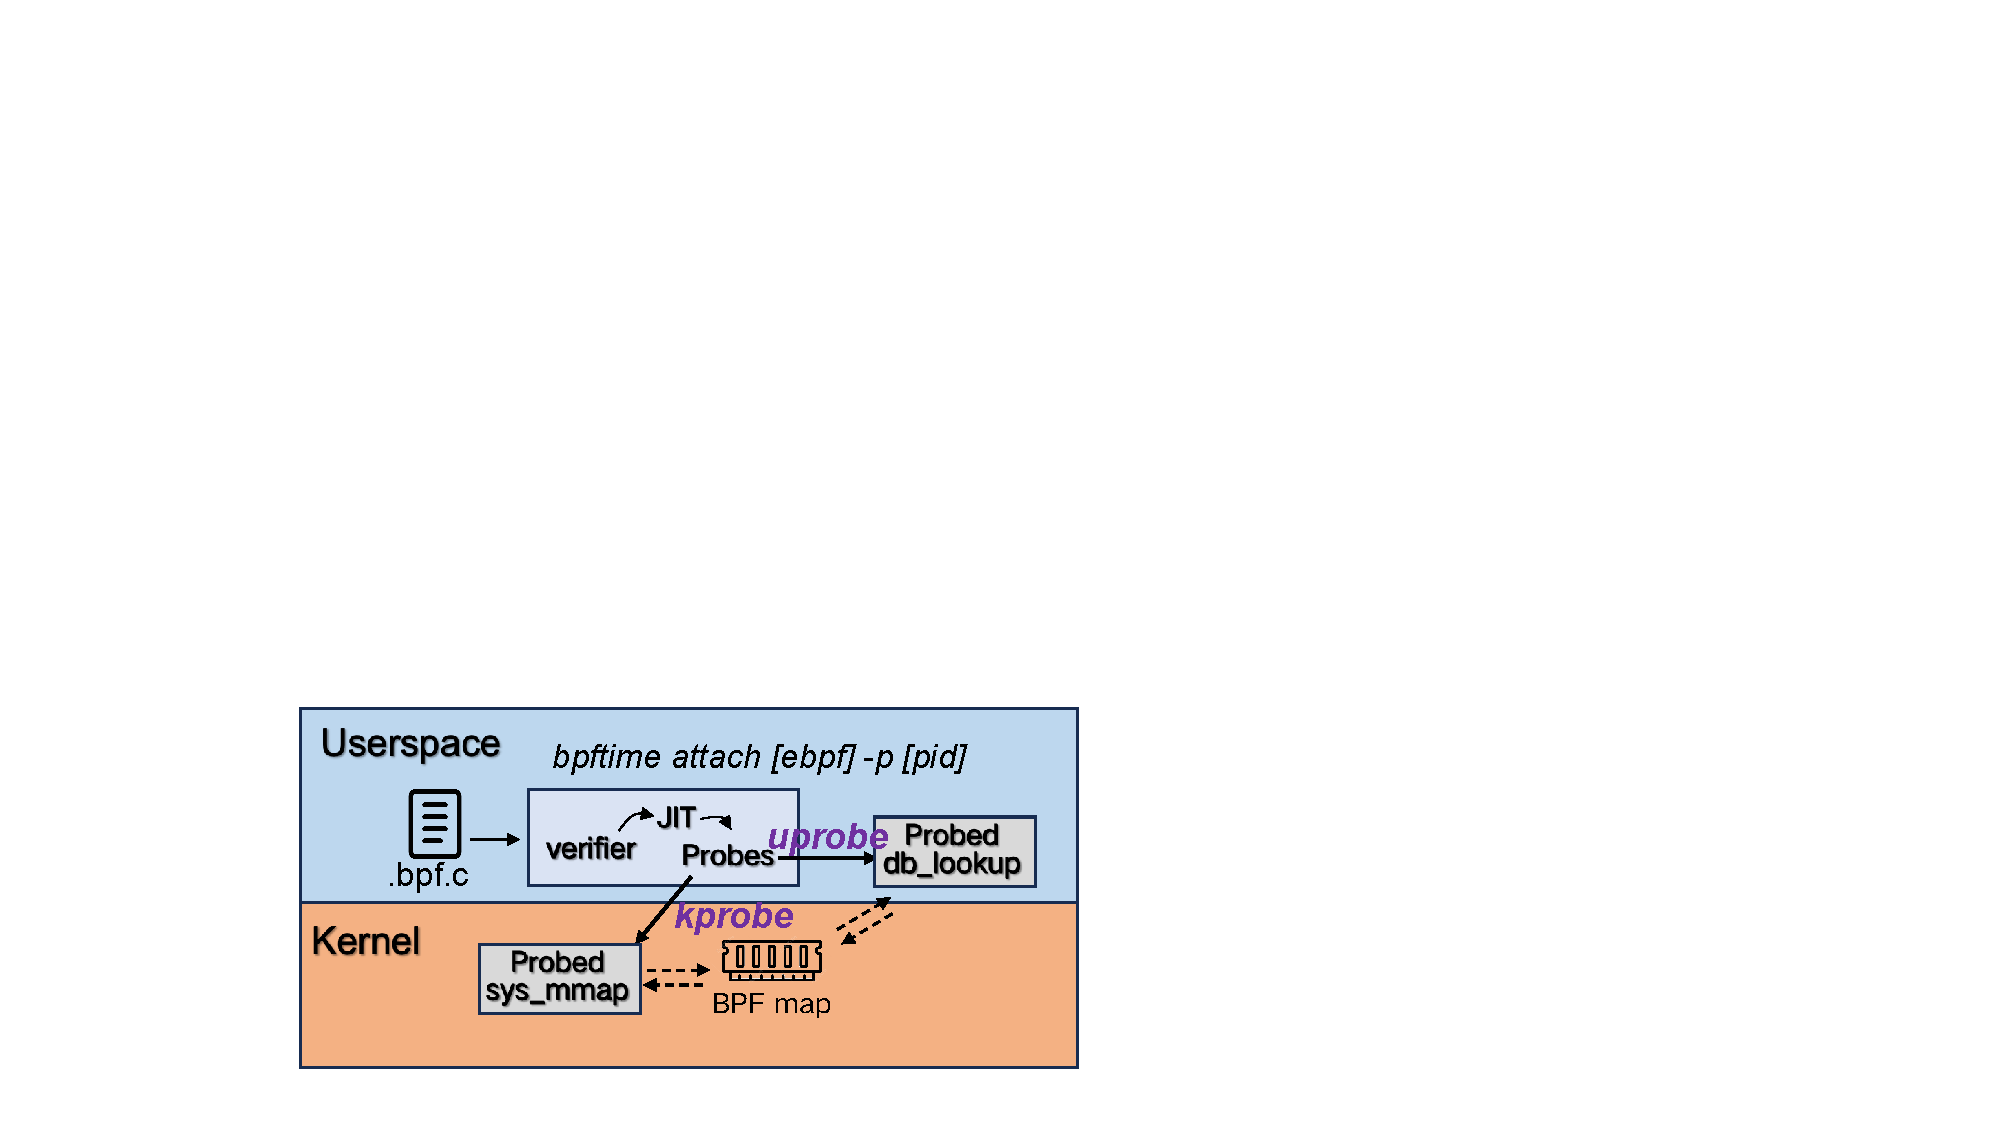
\includegraphics[width=\columnwidth]{img/bpf.pdf}
\caption{Userspace BPF Diagram}\label{fig:bpf}
\end{figure}

\subsection{PTX Just-In-Time Compilation}
PTX (Parallel Thread Execution) is an intermediate representation for NVIDIA GPUs that is faster than tools like NVBit~\cite{villa2019nvbit,kamath2021iguard}. PTX Just-In-Time (JIT) compilation~\cite{huang2024parallelgpuos,han2024microsecond} converts PTX to machine code at runtime, enabling dynamic instrumentation by intercepting and modifying PTX instructions. This allows embedding profiling or analytics logic with minimal overhead. Operating at a higher-level IR, PTX JIT achieves better performance than binary-level frameworks by producing optimized, architecture-specific code.

\subsection{GPU Scheduling and Security}
Confidential computing for GPUs aims to protect model workloads. Soter~\cite{shen2022soter} uses a CPU enclave but incurs high latency. Honeycomb~\cite{mai2023honeycomb} adds a trusted software layer with runtime checks, also impacting performance. Other approaches like microsecond-scale scheduling~\cite{han2022microsecond} involve kernel modifications. In contrast, PipeLLM~\cite{tan2025pipellm} uses speculative pipelining of encryption and data transfers to reduce confidentiality overhead without code or hardware changes.

\subsection{Motivation}\label{sec:motivation}
Existing GPU instrumentation tools like CUPTI~\cite{cupti} and NVBit~\cite{villa2019nvbit} often have high overhead. eBPF is a lightweight alternative for CPU-centric tasks~\cite{ghigoff2021bmc,zhong2022xrp,yang2023lambda}, but it lacks direct GPU insight. Modern GPU workloads require real-time, on-the-fly instrumentation without halting kernels. As shown in \Cref{fig:latency}, current tools cannot inject logic into running kernels. To address this, we introduce \sys, a framework that extends eBPF to GPUs via runtime PTX injection. \sys{} compiles eBPF to PTX, injects it into active kernels, and uses user-space probes and shared memory for low-overhead instrumentation, enabling dynamic observability for GPU workloads.

\begin{figure} \centering 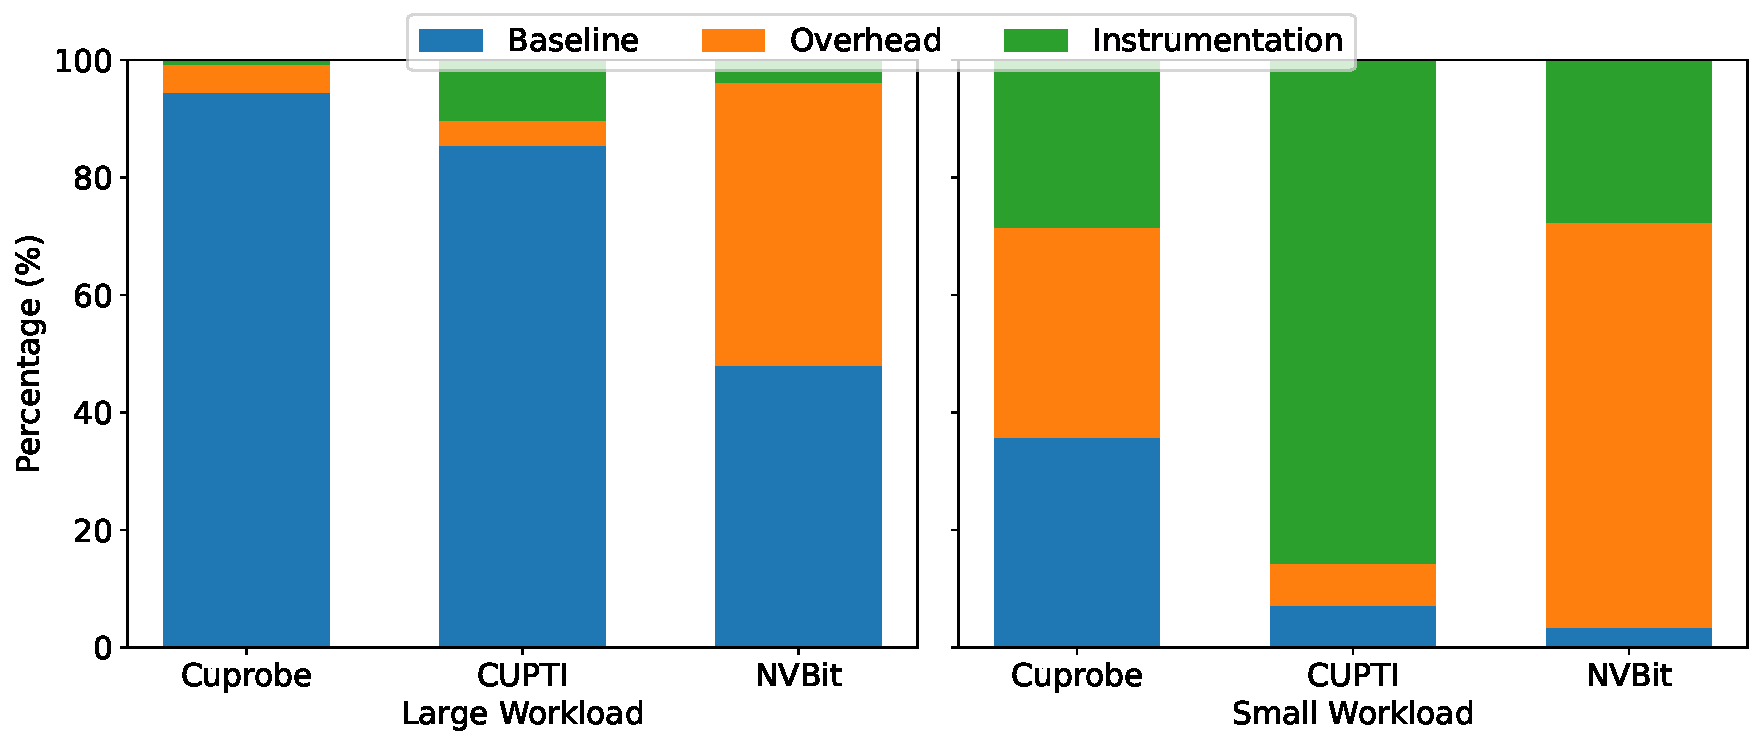
\includegraphics[width=0.5\textwidth]{img/motivation.pdf} \caption{Null Tool Runtime and Instrumentation Overhead Breakdown} \label{fig:latency} \end{figure}
